%% Article SC-Reborn pour International Journal of Production Economics
%% MATÉRIEL SUPPLÉMENTAIRE : compléments retirés du manuscrit principal (manuscrit.tex).
%% Les renvois « section S… » du manuscrit pointent vers les sections de ce document.

\documentclass[11pt,a4paper]{article}
\usepackage[T1]{fontenc}
\usepackage[english]{babel}
\usepackage[margin=2.3cm]{geometry}
\usepackage[authoryear,longnamesfirst]{natbib}
\usepackage{amsmath,amssymb}
\usepackage{booktabs,tabularx}
\usepackage{capt-of}
\usepackage{graphicx}
\usepackage{xcolor}
\usepackage{tikz}
\usetikzlibrary{arrows.meta,positioning,fit,backgrounds,calc,patterns}
\usepackage[hidelinks]{hyperref}
% Réglages communs au manuscrit et au matériel supplémentaire : couleurs, colonnes, champs à compléter.
% Couleurs des figures (politiques de gestion et paliers du réseau bayésien)
\definecolor{polnone}{HTML}{5C5B56}
\definecolor{poltard}{HTML}{EDA100}
\definecolor{polprud}{HTML}{EB6834}
\definecolor{polreac}{HTML}{2A78D6}
% Couleurs des politiques dans l'application Isomorph-Reborn
\definecolor{appnone}{HTML}{9CA3AF}
\definecolor{appprud}{HTML}{2563EB}
\definecolor{appreac}{HTML}{DC2626}
\definecolor{apptard}{HTML}{16A34A}
\definecolor{palctx}{HTML}{8A8984}
\definecolor{palpol}{HTML}{2A78D6}
\definecolor{palrep}{HTML}{EDA100}
\definecolor{palmec}{HTML}{1BAF7A}
\definecolor{palres}{HTML}{EB6834}
\usepackage{pgfplots}
\pgfplotsset{compat=1.17}
\newcolumntype{L}{>{\raggedright\arraybackslash}X}
\newcolumntype{P}[1]{>{\raggedright\arraybackslash}p{#1}}
% Champs restant à compléter avant la soumission (en bleu)
\newcommand{\acompleter}[1]{\textcolor{blue}{#1}}

% Renvois du manuscrit vers le matériel supplémentaire (numérotation S1, S2, ... fixée dans supplement.tex)
\newcommand{\voirSM}[1]{voir le matériel supplémentaire, section~#1}


% Numérotation propre au matériel supplémentaire : S1, S2... pour les sections, figures, tableaux et équations
\renewcommand{\thesection}{S\arabic{section}}
\renewcommand{\thefigure}{S\arabic{figure}}
\renewcommand{\thetable}{S\arabic{table}}
\renewcommand{\theequation}{S\arabic{equation}}
\setcounter{tocdepth}{2}

\title{Digital twin and causal Bayesian control of supply chain resilience\\[4pt]
\large Supplementary material}
\author{Authors anonymized for review}
\date{}

\begin{document}
\maketitle

\noindent This document complements the main manuscript and follows the order of its sections. It first presents a detailed view of the approach (S1), then the detailed literature review (S2), the modeling details for the three blocks, Simulate (S3), Measure (S4), and Learn (S5), the additional results (S6), and the instructions for reproducing the figures (S7). Figures, tables, and equations are numbered S1, S2, etc.; references to the main manuscript are marked as such.

\tableofcontents

\section{Detailed view of the approach}
\label{sec:S1}

Figure~\ref{fig:demarche-detail} details the approach summarized in Figure~1 of the main manuscript. For each of the three blocks, it specifies the inputs, the processing steps, and the outputs: the generation of labeled crises and their four versions (Simulate), the fitting of the resilience curve and the computation of the indicators (Measure), and the learning of the causal Bayesian network and its three uses (Learn). Thumbnails show a trajectory, a fitted curve, and the structure of the learned network.

\begin{center}\begin{minipage}{\textwidth}\centering
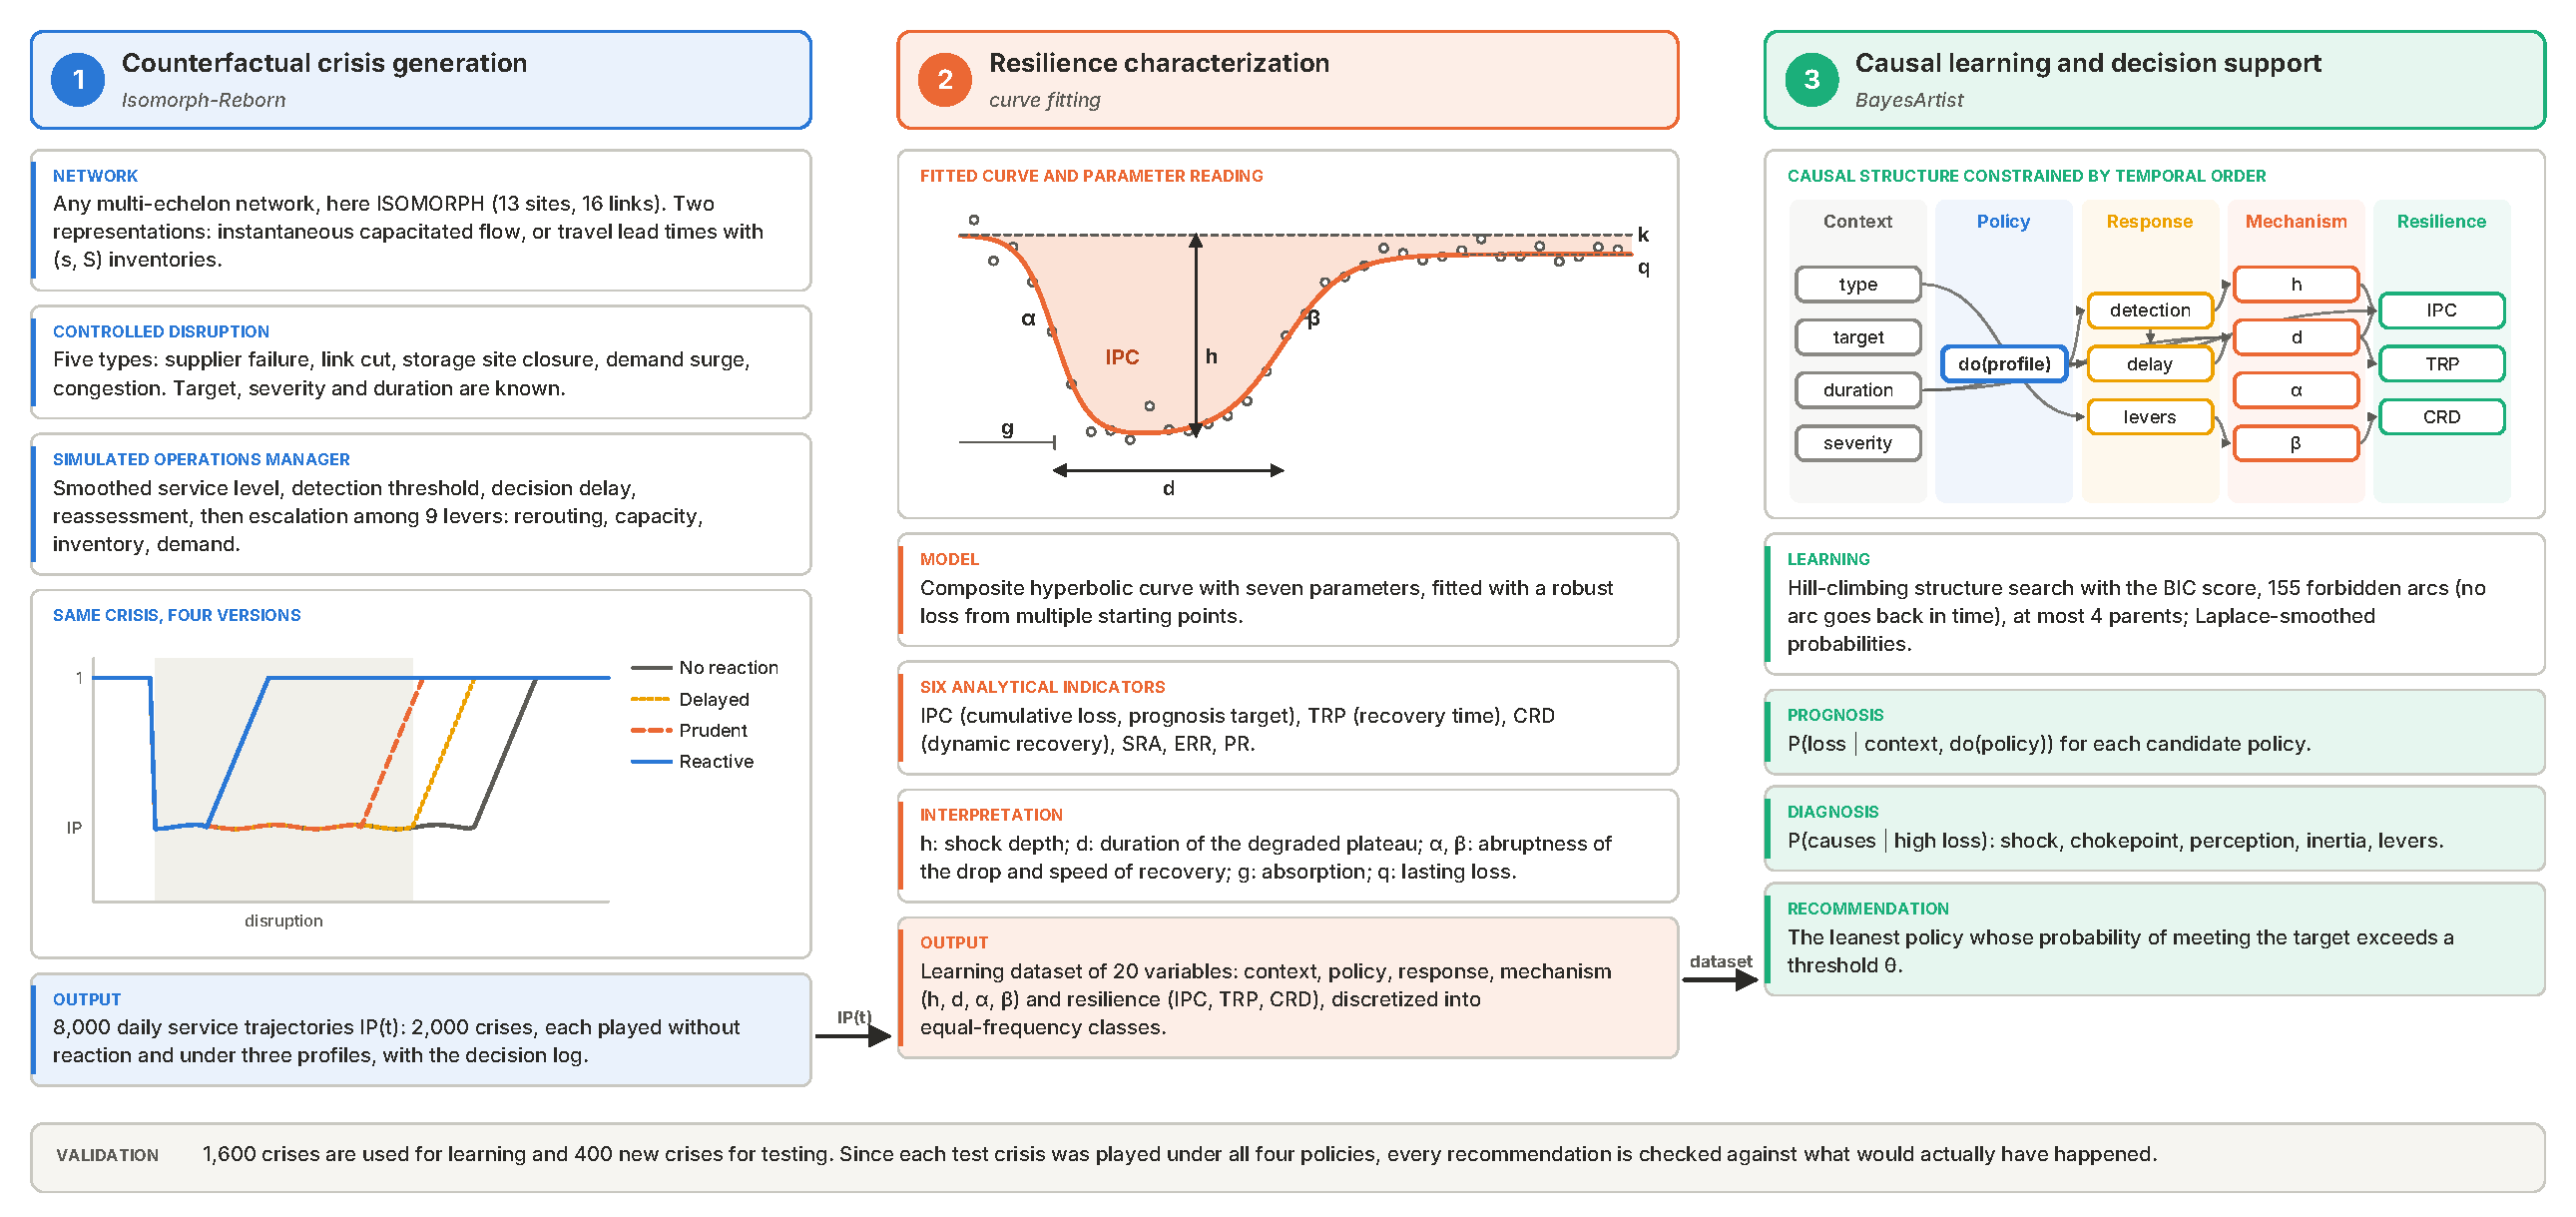
\includegraphics[width=\textwidth]{figures/Fig1_approach_EN.pdf}
\captionof{figure}{Detailed three-block approach: inputs, processing steps, and outputs of each block.}\label{fig:demarche-detail}
\end{minipage}\end{center}

\section{Detailed literature review}
\label{sec:S2}

This section expands, stream by stream, the state of the art summarized in Section~2 of the main manuscript; Table~1 of the main manuscript gives its synthesis.

\subsection{Supply chain resilience: definitions and resilience curve}
\label{sec:ea-mesure}

Literature reviews agree on defining resilience as the ability of a supply chain to prepare for disruptions, respond to them, and recover from them \citep{tukamuhabwa2015, kamalahmadi2016}. This definition has been formalized mathematically from the performance trajectory, which describes the drop and then the recovery of a supply chain subjected to a disruption \citep{rahiel2026in4pl, rahiel2026these}. It has been applied to the hospital supply chain \citep{rahiel2025esd} and extended by a probabilistic modeling of severe disruptions upstream of the network \citep{rahiel2026codit}. \citet{kamalahmadi2016} organize resilience into three phases: anticipation, resistance, and then recovery and response. Their review of one hundred articles also shows that measurement remains the neglected part of the field: only eight studies address it, against sixty-eight on the principles of resilience. Some measures rely on the perception of the actors, such as the survey scale of \citet{chowdhury2017}; it informs on the capabilities of a firm, not on the course of a given crisis.

The other family of measures starts from performance observed over time. \citet{bruneau2003} associate the loss of resilience with the area between nominal performance and degraded performance, until the return to equilibrium (Fig.~\ref{fig:courbe}). Replaying the same crisis with no reaction, then with a decision taken at $t_d$, isolates the effect of this decision (hatched area): the return to equilibrium occurs at $t_r'$ with the decision and at $t_r$ with no reaction. This counterfactual reading of the curve, with and without a decision, is borrowed from \citet{rahiel2026in4pl}. In the logistics field, \citet{sheffirice2005} describe an eight-phase disruption profile, from preparation to long-term impact, which holds whatever measure is used: sales, production, profit, or customer service. \citet{henry2012} generalize the idea by defining resilience as a function of time that accounts for the event, the restoration of components, and the strategy adopted. \citet{zobel2011} show that two crises with the same area are not equivalent for the decision maker, who trades off the magnitude of the initial impact against the duration of recovery. The reviews by \citet{hosseini2016} and \citet{hosseini2019tre} survey these measures, the latter according to the capability involved: absorbing, adapting, or recovering.

\begin{center}
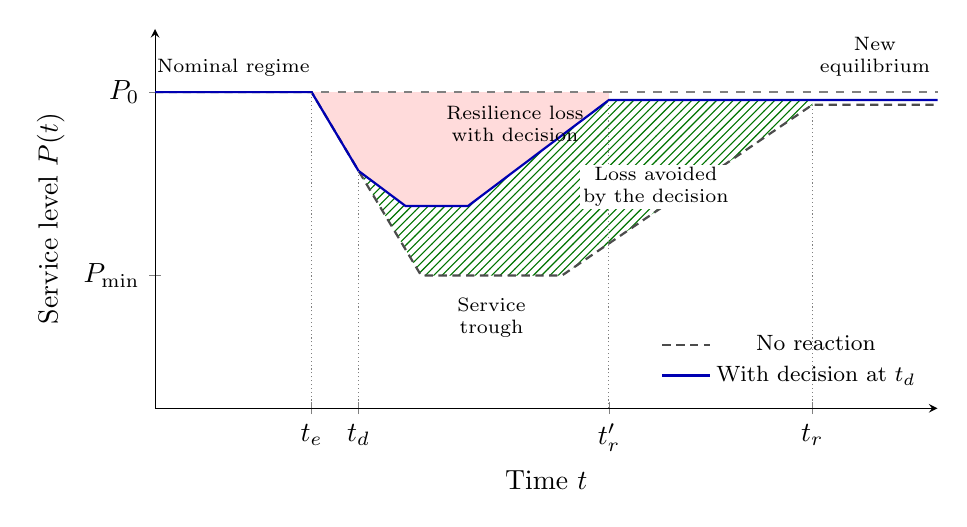
\begin{tikzpicture}
\begin{axis}[
  width=0.95\textwidth, height=6.4cm,
  xmin=0, xmax=100, ymin=0, ymax=1.2,
  axis lines=left,
  xlabel={Time $t$}, ylabel={Service level $P(t)$},
  xtick={20,26,58,84},
  xticklabels={$t_e$,$t_d$,$t_r'$,$t_r$},
  ytick={0.42,1}, yticklabels={$P_{\min}$,$P_0$},
  every axis plot/.append style={thick},
  legend style={font=\footnotesize, draw=none, fill=none, at={(0.99,0.03)}, anchor=south east},
  clip=false]
  % Resilience loss with decision (between the nominal level and the trajectory with decision)
  \addplot[fill=red!14, draw=none, forget plot] coordinates
    {(20,1) (26,0.751) (32,0.64) (40,0.64) (58,0.975) (58,1) (20,1)};
  % Loss avoided by the decision (between the two trajectories)
  \addplot[pattern=north east lines, pattern color=green!45!black, draw=none, forget plot] coordinates
    {(26,0.751) (32,0.64) (40,0.64) (58,0.975) (84,0.975) (84,0.96) (52,0.42) (34,0.42) (26,0.751)};
  % Nominal level
  \addplot[dashed, gray, forget plot] coordinates {(0,1) (100,1)};
  % Trajectory with no reaction
  \addplot[black!70, densely dashed] coordinates
    {(0,1) (20,1) (34,0.42) (52,0.42) (84,0.96) (100,0.96)};
  \addlegendentry{No reaction}
  % Trajectory with a decision taken at t_d
  \addplot[blue!70!black] coordinates
    {(0,1) (20,1) (26,0.751) (32,0.64) (40,0.64) (58,0.975) (100,0.975)};
  \addlegendentry{With decision at $t_d$}
  % Reference lines
  \draw[gray, densely dotted] (axis cs:20,0) -- (axis cs:20,1);
  \draw[gray, densely dotted] (axis cs:26,0) -- (axis cs:26,0.751);
  \draw[gray, densely dotted] (axis cs:58,0) -- (axis cs:58,0.975);
  \draw[gray, densely dotted] (axis cs:84,0) -- (axis cs:84,0.96);
  % Labels
  \node[font=\scriptsize, align=center] at (axis cs:46,0.90) {Resilience loss\\with decision};
  \node[font=\scriptsize, align=center, fill=white, inner sep=1pt] at (axis cs:64,0.70) {Loss avoided\\by the decision};
  \node[font=\scriptsize, anchor=south] at (axis cs:10,1.02) {Nominal regime};
  \node[font=\scriptsize, anchor=north, align=center] at (axis cs:43,0.38) {Service\\trough};
  \node[font=\scriptsize, anchor=south, align=center] at (axis cs:92,1.02) {New\\equilibrium};
\end{axis}
\end{tikzpicture}
\captionof{figure}{Service level after a disruption at $t_e$, with and without a decision at $t_d$ (illustrative diagram, after \citet{rahiel2026in4pl}).}\label{fig:courbe}
\end{center}

Several studies derive indicators from this trajectory that can be used for decision making. \citet{spiegler2012} measure resilience by the integral of the time-weighted deviation in inventory and shipment levels and show that a more resilient chain has higher production costs: resilience has a price. \citet{simchilevi2015} assess risk exposure at Ford from the recovery time of each site, postponing the estimation of probabilities until after that of the effects; they observe that the impact of a disruption often depends less on its cause than on its duration. \citet{behzadi2020} show that the choice of measure changes the investment strategy selected and propose the discounted value of lost profit. \citet{dixit2020} relate resilience before and after a disaster to structural network parameters such as density, centrality, and connectivity.

A recent formalization describes the whole curve by an explicit function rather than by indicators computed point by point. A composite function of hyperbolic tangents with seven parameters covers the complete disruption cycle and yields six indicators, including cumulative loss, recovery speed, and adaptive robustness \citep{rahiel2026in4pl, rahiel2026these}. These measures, like the previous ones, apply to a curve that has already been observed. None of them says how to obtain comparable curves in large numbers, for varied crises and different responses.

% ---------------------------------------------------------------------
\subsection{Mitigation and contingency strategies against disruptions}
\label{sec:ea-strategies}

The literature distinguishes measures taken before the disruption, called mitigation, from those taken once it occurs, called contingency. \citet{tang2006} classifies the former according to whether they concern supply, demand, product, or information. \citet{tomlin2006} formalizes the choice for one product and two suppliers, one cheap but unreliable, the other reliable but more expensive. The optimal strategy then depends on the supplier's availability rate and on the nature of the disruptions, frequent and short or rare and long. Contingent rerouting is often part of it. \citet{sheffirice2005} contrast redundancy, a mere cost as long as no crisis occurs, with flexibility, which provides an advantage even in normal times.

Quantitative studies clarify the role of each lever. For \citet{lucker2019}, inventory acts as prevention and reserve capacity as reaction; their optimal levels depend on the type of product and of supply chain. Safety stock has also been studied as a resilience lever in the hospital supply chain, against seasonal activity peaks \citep{rahiel2025esd}. \citet{hosseini2019ijpe} combine proactive and reactive strategies in supplier selection and order allocation. \citet{ivanov2016tre} compare several proactive configurations and several recovery policies in terms of service level and costs. Faced with a long disruption such as the COVID-19 pandemic, \citet{ivanovdolgui2021ijpe} conclude that adaptation capabilities matter most.

The economic dimension runs through these studies. \citet{aldrighetti2021} review the costs of proactive investments and of recovery in network design models. \citet{klibi2012ijpe} show, in a design problem, that how well the model anticipates the operational response of users strongly affects the result, and they stress that these response mechanisms have received little modeling attention.

These studies establish a repertoire of decisions: inventory, backup supply, rerouting, capacity, and demand allocation. However, the decisions are most often fixed in advance, by optimization or by case analysis. Their triggering as the crisis unfolds, with the detection, decision, and implementation delays of a real operations manager, remains little modeled, as does the comparison of several management policies facing the same hazard.

% ---------------------------------------------------------------------
\subsection{Simulation of disruptions and recovery}
\label{sec:ea-simulation}

Simulation has become the standard tool for studying the propagation of disruptions in networks, known as the \textit{ripple effect}. \citet{schmitt2012} simulate a real consumer goods network to compare supply and demand interruption risks and the effect of placing inventory at several echelons. \citet{ivanov2017} presents a simulation model of a multi-echelon chain subject to capacity losses and stresses that simulation covers blind spots of optimization. Applied to COVID-19, the same approach shows that the timing of site closures and reopenings, echelon by echelon, can weigh more on the impact than the duration of the upstream disruption or the speed of propagation \citep{ivanov2020}. Nor does the crisis end when sites reopen: accumulated delays and backlogs persist. \citet{ivanov2019cie} shows that a recovery policy, which provides a gradual transition from contingency to normal operation, mitigates part of them.

On the methodological side, \citet{macdonald2018} combine design of experiments (DoE) and discrete-event simulation to build theory, varying the interval between disruptions, connectivity, and buffer stocks. Timed discrete-event formalisms also make it possible to bound analytically the execution times of a chain subject to uncertain durations and then, when a disruption occurs, to choose the fastest reconfiguration scenario \citep{rajah2025}. Network structure also matters \citep{kim2015}: a set of network characteristics describes resilience better than the network type alone \citep{li2020}.

Scenarios themselves can be generated systematically. \citet{klibi2012ejor} characterize the hazards and vulnerabilities of the network, model the arrival, intensity, and duration of incidents, and then assess their consequences in terms of damage and recovery time; random sampling then produces plausible scenarios for network design. Digital twins represent the state of the network continuously \citep{ivanovdolgui2021ppc}, and \citet{ivanov2023} turns the digital twin into a stress-testing tool. The MARE framework covers the four stages of disruption management (monitor, assess, recover, and assess the recovery) and compares the restoration achieved by several recovery strategies \citep{ramzy2022}. Finally, ISOMORPH, the first public digital twin of a multi-echelon logistics network, provides reference trajectories for forecasting; closed-loop control, that is, a decision that reacts to the state of the network, appears only among the envisaged extensions \citep{zhang2026isomorph}.

These simulators bring out what aggravates or mitigates a crisis. But they are designed to study a network or a case, not to produce a dataset of comparable crises. Strategies are fixed by the scenario. None of the studies reviewed systematically replays the same hazard with no reaction and then under several management policies.

% ---------------------------------------------------------------------
\subsection{Causal Bayesian networks in supply chain management}
\label{sec:ea-rb}

Bayesian networks have become a preferred tool for representing dependencies between risks, strategies, and consequences. The review by \citet{hosseiniivanov2020} highlights three strengths: inference in both directions, from cause to effect to simulate a disruption and from effect to cause to identify which levers to strengthen; the combination of expert knowledge and data; and the ability to work with little data. \citet{garvey2015} and \citet{ojha2018} model risk propagation in the network, the latter deriving risk exposure and resilience indices. \citet{hosseiniivanov2022aor} base a resilience measure on supplier vulnerability and recoverability. The decision question is addressed by \citet{qazi2018}, who couple a Bayesian network with expected utility to select mitigation strategies. The probabilities of their model are elicited from company staff through interviews and workshops. An upstream probabilistic layer has also been proposed to model the resilience of a network under severe disruptions \citep{rahiel2026codit}.

The structure of these networks is most often set by experts; it can also be learned from data, through a score that rewards fit and penalizes complexity or through independence tests \citep{koller2009, hosseiniivanov2020}. The two sources can be combined \citep{heckerman1995}. For such a model to recommend a decision, the effect of that decision must still be identifiable. In the sense of \citet{pearl2009}, a decision is an intervention: its consequence cannot be read from a simple observed correlation, because the operations manager reacts all the more strongly as the crisis is more severe.

Yet the necessary data are lacking. \citet{hosseiniivanov2020} note that major disruptions are rare, so that the available data are insufficient to quantify resilience. Even at a large manufacturer, data on lower-tier suppliers remain hard to obtain \citep{simchilevi2015}. Learning studies therefore rely on internal industrial data, such as the Ford time series used by \citet{do2024} to forecast delivery delays. These records are not public and contain neither the label of the decision taken nor the counterfactual, that is, what would have happened without it: each crisis occurs only once, with a single response.

% ---------------------------------------------------------------------

\section{Scenario generator details (Simulate)}
\label{sec:S3}

\subsection{Reference networks}
\label{sec:S3.1}

Two networks serve as references (Table~\ref{tab:reseaux}). The parametric network has three echelons: three factories, nine warehouses, and one final customer. Each warehouse is supplied by a main factory, by a backup factory through a lower-capacity link, and, for one warehouse in three, by a third factory. Redundancy is therefore partial by construction. The loss of a warehouse's main route can only be partly offset by its fallback routes, as in most real networks, where dual sourcing remains costly.

The ISOMORPH network keeps the original topology (Fig.~\ref{fig:d2}): thirteen cities connected by sixteen links, with a hub and five intermediate echelons between the sources and the customer. Since the original file does not set all the required quantities, three assumptions complete its description. The capacity of each link is drawn within plus or minus 10\% of its original value. The production capacity of each source is set at 0.8 times the cumulative capacity of its outgoing links; at 1.0, production could never be a capacity bottleneck and shifting load to unaffected production sites would have no effect. Finally, the last mile is assumed to be unlimited; the last two storage sites before the customer then have neither their own capacity nor a limited outgoing link and are beyond the reach of the shipping levers.

\begin{center}
% Figure: original ISOMORPH network by echelon (data: reseau_isomorph-originel.json)
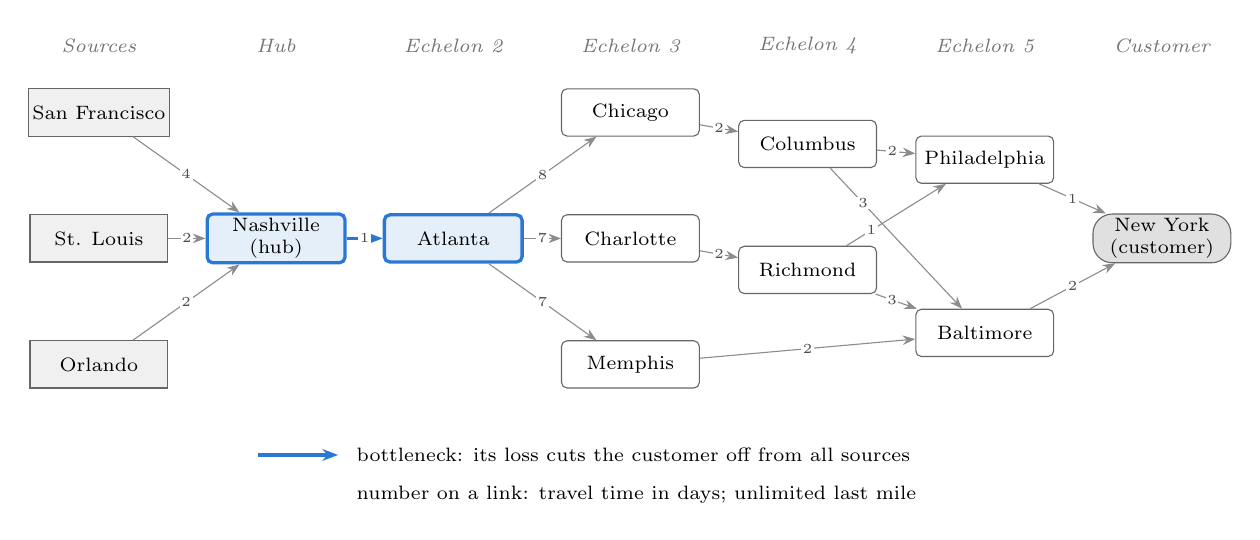
\begin{tikzpicture}[x=2.25cm,y=1cm,
  site/.style={draw=black!60, rounded corners=2pt, fill=white, font=\scriptsize, minimum width=1.75cm, minimum height=0.6cm, align=center, inner sep=1.5pt},
  usine/.style={site, fill=black!6, rounded corners=0pt},
  oblige/.style={site, draw=polreac, very thick, fill=polreac!12},
  client/.style={site, rounded corners=7pt, fill=black!12},
  arc/.style={-{Stealth[length=1.6mm]}, black!45, thin},
  arcob/.style={-{Stealth[length=2mm]}, polreac, very thick},
  delai/.style={font=\tiny, fill=white, inner sep=0.6pt, text=black!70}]
  % echelons
  \node[usine] (SF) at (0, 1.6) {San Francisco};
  \node[usine] (SL) at (0, 0)   {St. Louis};
  \node[usine] (OR) at (0,-1.6) {Orlando};
  \node[oblige] (NA) at (1, 0) {Nashville\\(hub)};
  \node[oblige] (AT) at (2, 0) {Atlanta};
  \node[site] (CH) at (3, 1.6) {Chicago};
  \node[site] (CT) at (3, 0)   {Charlotte};
  \node[site] (ME) at (3,-1.6) {Memphis};
  \node[site] (CO) at (4, 1.2) {Columbus};
  \node[site] (RI) at (4,-0.4) {Richmond};
  \node[site] (PH) at (5, 1.0) {Philadelphia};
  \node[site] (BA) at (5,-1.2) {Baltimore};
  \node[client] (NY) at (6, 0) {New York\\(customer)};
  % links and travel times (days)
  \draw[arc] (SF) -- node[delai]{4} (NA);
  \draw[arc] (SL) -- node[delai]{2} (NA);
  \draw[arc] (OR) -- node[delai]{2} (NA);
  \draw[arcob] (NA) -- node[delai]{1} (AT);
  \draw[arc] (AT) -- node[delai]{8} (CH);
  \draw[arc] (AT) -- node[delai]{7} (CT);
  \draw[arc] (AT) -- node[delai]{7} (ME);
  \draw[arc] (CH) -- node[delai]{2} (CO);
  \draw[arc] (CT) -- node[delai]{2} (RI);
  \draw[arc] (CO) -- node[delai,pos=0.4]{2} (PH);
  \draw[arc] (CO) -- node[delai,pos=0.25]{3} (BA);
  \draw[arc] (RI) -- node[delai,pos=0.25]{1} (PH);
  \draw[arc] (RI) -- node[delai,pos=0.4]{3} (BA);
  \draw[arc] (ME) -- node[delai]{2} (BA);
  \draw[arc] (PH) -- node[delai]{1} (NY);
  \draw[arc] (BA) -- node[delai]{2} (NY);
  % echelons
  \foreach \x/\t in {0/Sources, 1/Hub, 2/{Echelon 2}, 3/{Echelon 3}, 4/{Echelon 4}, 5/{Echelon 5}, 6/Customer}
    \node[font=\scriptsize\itshape, text=black!55] at (\x, 2.45) {\t};
  % legend
  \begin{scope}[shift={(0,-2.75)}]
    \draw[arcob] (0.9,0) -- (1.35,0);
    \node[font=\scriptsize, anchor=west] at (1.4,0) {bottleneck: its loss cuts the customer off from all sources};
    \node[font=\scriptsize, anchor=west] at (1.4,-0.5) {number on a link: travel time in days; unlimited last mile};
  \end{scope}
\end{tikzpicture}

\captionof{figure}{Original ISOMORPH network shown by echelon, from the three sources to the customer.}\label{fig:d2}
\end{center}

\begin{table}[htbp]
\caption{Characteristics of the two reference networks (nominal values).}
\label{tab:reseaux}
\footnotesize
\begin{tabularx}{\textwidth}{@{}P{4.2cm}LL@{}}
\toprule
\textbf{Item} & \textbf{Parametric network} & \textbf{ISOMORPH network} \\
\midrule
Sites and echelons & 3 factories, 9 warehouses, 1 customer & 13 cities, 16 links, 1 hub, 5 intermediate echelons \\
Production capacity of a source (units per day) & 200 to 320 & 0.8 times the capacity of its outgoing links \\
Link capacity (units per day) & Main route 60 to 110; backup route 15 to 35; third route 10 to 20 & Original value $\pm$10\%; unlimited last mile \\
Shipping capacity of a storage site (units per day) & 50 to 100 & Carried by the outgoing links \\
Transit time, temporal representation (days) & 0 by default, adjustable & 1 to 8 (original values) \\
Production lead time, temporal representation (days) & 0 by default, adjustable & 0 by default, adjustable \\
Share of critical items in demand & 15\% to 45\% & 15\% to 45\% \\
Daily demand fluctuation & $\pm$3\% to $\pm$8\% & $\pm$3\% to $\pm$8\% \\
\bottomrule
\end{tabularx}
\end{table}

In the flow representation, the deliverable volume $F(t)$ on a given day is the maximum quantity the network can carry from the sources to the customer given all its capacities, degraded or reinforced on that day. This formulation reveals the capacity bottlenecks. It is often the shipping capacity of storage sites, rather than production, that limits service. In the temporal representation, $F(t)$ denotes the volume that the movement of material and the inventories actually allow to be delivered on that day.

\subsection{Temporal representation: lead times and inventory policy}
\label{sec:S3.2}

The flow representation assumes that material moves instantaneously and that no inventory stands between the capacities and the customer. The temporal representation removes these two assumptions. Each link has a transit time and each production site a production lead time, expressed in whole days. Orders travel upstream instantaneously, but material takes the time of these lead times to move down to the customer. Each storage site manages its inventory with an (s, S) inventory policy \citep{scarf1960}: when its inventory position, on-hand inventory plus material in transit, falls below the reorder point s, it orders the quantity that brings it back up to level S.

The levels $s_{i}$ and $S_{i}$ of a storage site i are expressed in days of cover of its own nominal throughput, to which is added the inventory that is necessarily in transit to it:

\begin{equation}
s_i = c_s\,\Phi_i + \sum_{a \in A_i} (L_a + P_a)\, f_a, \qquad S_i = c_S\,\Phi_i + \sum_{a \in A_i} (L_a + P_a)\, f_a
\label{eq:S1}
\end{equation}

$\Phi_{i}$ denotes the nominal throughput of site i, the sum of the nominal throughputs of its supply links for the reference demand (Section~3.2 of the main manuscript), $c_{s}$ and $c_{S}$ the covers in days, 3 and 10 days by default, $A_{i}$ the set of links that supply site i, $L_{a}$ the transit time of link a, $P_{a}$ the production lead time of its origin site, and $f_{a}$ its nominal throughput. The second term applies Little's law \citep{little1961} link by link. It sizes the material in transit so that, in steady state, on-hand inventory matches the chosen cover, however heterogeneous the supply lead times. Relating the cover to the throughput of each site, rather than to an equal share of demand, is essential in a serial network. Otherwise, a hub through which the entire flow passes would receive the same cover as a secondary warehouse and the network would stop delivering even without a disruption. When the network description sets the levels of a site, these levels are kept.

Three rules complete the representation. Each day, a storage site first serves the day's requirements and then the replenishment of downstream sites. Allocation favors the main link over backup links. Critical and ordinary items are aggregated in inventory, and priority to critical items applies only to customer service. Finally, links to the customer are served the same day. With a lead time on these links, the customer would receive today what it ordered the day before and the indicator would drop with every day-to-day increase in demand, even without a disruption; it would then measure demand noise rather than network availability.

Before any observation, the network is simulated without disruption during a 60-day burn-in, which brings inventories and material in transit to their steady state. This burn-in is common to the four versions of the same crisis.

The two representations are nested. With zero lead times, the temporal representation reproduces the flow representation almost exactly, with a mean service level gap between 0.00025 and 0.002 depending on the cases tested. With lead times, however, inventories deeply alter the network's response to disruptions, to an extent that depends on the cover and on the nature of the disruption; Section~S6.4 analyzes this sensitivity.

\subsection{Disruptions and calibration of the reference demand}
\label{sec:S3.3}

The link cut illustrates an often underestimated phenomenon, because the loss of a main route is not limited to the volume it carried. The storage site deprived of its usual supply must reorganize in a hurry, which degrades its own shipping capacity. Its backup routes, overloaded, also lose efficiency. The disruption thus propagates beyond its target. Cuts and closures are treated as near-total outages, hence a higher severity; the duration of any disruption ranges from 3 to 15 days. In the temporal representation, these capacity reductions apply in the same way, but their effect on the customer is cushioned by inventories and delayed by the material already in transit.

The effect of a disruption depends as much on its severity as on the strain under which the network operates. A network with slack absorbs a disruption that would break a saturated network. To control this factor, the reference demand of each scenario is set according to the volume still deliverable during the incident, using a strain rate $u$ drawn between 0.85 and 1.15:

\begin{equation}
D_{max} = \min\left(\frac{u \cdot F_{inc}}{m_{inc}},\ \frac{0.995 \cdot F_{nom}}{1 + \varepsilon}\right)
\label{eq:S2}
\end{equation}

$F_{\mathrm{inc}}$ and $F_{\mathrm{nom}}$ denote the deliverable volume during the incident and under normal operation, $m_{\mathrm{inc}}$ the demand multiplier during the incident (1 + 2s for a demand surge, 1 otherwise), and $\varepsilon$ the amplitude of the daily fluctuation. $D_{\max}$ is the highest demand that the network serves both during the incident (up to the strain $u$) and without degradation under normal operation. The volumes $F_{\mathrm{inc}}$ and $F_{\mathrm{nom}}$ are obtained by a maximum flow computation (Edmonds-Karp algorithm). The factor $0.995$ leaves a margin of $0.5\%$ below nominal capacity. This margin does not follow from any theory; it is a simulator parameter set by trial. Initially set at $0.97$, it was tightened to $0.995$ because a wider margin flattened the effect of a link cut in a redundant network. A strain below 1 only reduces the network's margin; a strain above 1 creates an outright shortage. The second term guarantees, in the flow representation, that no degradation appears before the disruption, during an initial period of 10 days, so that any observed trough can be attributed to the crisis. In this representation, the reference demand $D_{0}$ equals $D_{\max}$, rounded to an integer.

In the temporal representation, $F_{\mathrm{inc}}$ and $F_{\mathrm{nom}}$ are measured by the simulation engine itself, under just-in-time flow: they are the volumes that the movement of material actually allows to be delivered, and they never exceed the maximum flow. The second term then no longer suffices to guarantee the absence of degradation, because lumpy replenishments and lead times can leave some demand unserved on a given day, even without a disruption. The reference demand is therefore checked by simulation. Each scenario is simulated without disruption, burn-in included, with its own series of fluctuations. The demand $D_{0}$ is the largest integer demand not exceeding $D_{\max}$ that is fully served every day:

\begin{equation}
D_0 = \max\left\{\, d \in \mathbb{N}^*,\ d \le D_{max} \;:\; \mathrm{PI}_d(t) = 1 \ \text{for every day } t \text{ simulated without disruption} \right\}
\label{eq:S3}
\end{equation}

$\mathrm{PI}_{d}(t)$ denotes the service level obtained under a reference demand $d$, with the levels s and S recomputed by Eq.~\eqref{eq:S1} for each demand tried. The search proceeds by bisection over the integers and can only lower $D_{\max}$; the value retained is always checked by simulation. When even a demand of one unit is not fully served, the inventory cover is too low given the fluctuations and lead times. The scenario then admits no nominal regime without degradation. In that case, the DoE is rejected rather than continued with an arbitrary demand. This feasibility condition directly links inventory cover, supply lead times, and demand variability.

\subsection{Remediation levers}
\label{sec:S3.4}

The nine levers of the simulated operations manager (Section~3.2 of the main manuscript) are detailed in Table~\ref{tab:d4}.

\begin{table}[htbp]
\caption{Remediation levers.}
\label{tab:d4}
\footnotesize
\begin{tabularx}{\textwidth}{@{}P{1.0cm}P{1.5cm}LLL@{}}
\toprule
\textbf{Lever} & \textbf{Family} & \textbf{Action} & \textbf{Nominal effect} & \textbf{Disruptions concerned} \\
\midrule
D1 & Rerouting & Load shift to unaffected production sites & +20\% capacity & Supplier failure, link cut, congestion \\
D2 & Rerouting & Shift to neighboring storage sites & +25\% shipping capacity & Link cut, storage site closure, congestion \\
D3 & Capacity & Overtime at the affected production site & 50\% of the loss recovered & Supplier failure \\
D4 & Capacity & Spot carrier on the affected link or site & 50\% of the loss recovered & Link cut, storage site closure \\
D5 & Capacity & Buffer warehouse & +15\% shipping capacity across the whole network & All \\
D6 & Inventory & Safety stock release & Flow: 30\% of demand, depleted in 10 days. Temporal: separate reserve released once, used only for unserved demand & All \\
D7 & Inventory & Inventory pre-positioning near the customer & Flow: 20\% of any loss offset. Temporal: s and S raised by 50\%, immediate order & Supplier failure, link cut, congestion \\
D8 & Demand & Prioritization of critical items & $-$25\% of ordinary demand served & All \\
D9 & Demand & Postponement of non-critical demand & 30\% of ordinary demand deferred & All \\
\bottomrule
\end{tabularx}
\end{table}

The levers do not all act in the same way. Rerouting and additional capacity restore or bypass lost capacity. Safety stock release brings temporary relief, which can produce a second trough when the stock runs out before the end of the crisis. Finally, demand levers improve the measured service level by giving up part of the ordinary demand; they reflect a service trade-off rather than a restoration of capacity, a distinction that should guide the interpretation of the recommendations.

In the temporal representation, the two inventory levers change mechanism. Inventory pre-positioning (D7) temporarily raises the s and S levels of the storage sites and triggers an immediate order. Safety stock release (D6) frees a safety reserve kept apart from ordinary inventory. This reserve is invisible to the ordering policy and serves only the demand that ordinary inventory could not meet.

This mechanism addresses an effect observed during development. When injected directly into ordinary inventory, the same quantity pushed some sites above their reorder point. They then skipped a replenishment and the missing requirement propagated up to the sources, which stood idle for a day during a supplier failure; the production capacity lost in this way was never recovered. In one measured case, the lever reduced the delivered volume instead of increasing it. An emergency intervention on inventories can therefore disrupt the replenishment signal it was meant to relieve. The separate reserve guarantees that safety stock release never reduces the delivered volume. Finally, the two inventory levers exclude storage sites that have no capacity of their own and unlimited outgoing links, since the levers have no hold on them.

\subsection{Design of experiments, strain level, and content of the observations}
\label{sec:S3.5}

The network characteristics, the nature, target, severity, and duration of the disruption, and the network strain are drawn independently for each scenario from a uniform distribution. Continuous quantities are drawn uniformly over the ranges described above: site and link capacities, share of critical items, amplitude of demand fluctuation, severity, duration (rounded to the day), and strain rate. The nature of the disruption is drawn uniformly among the five natures and its target among the eligible sites or links; a link cut, however, targets the main link of a site with probability 0.85, because cutting an already marginal backup route would have almost no effect. The daily demand fluctuation is also drawn uniformly, each day, between $-\varepsilon$ and $+\varepsilon$. In the absence of field data on crisis frequency, the uniform distribution gives the same weight to all plausible values and covers the scenario space without favoring any regime; the proportions observed in the dataset therefore describe this space and not the actual frequency of crises. All draws come from a seeded pseudo-random number generator. By contrast, the reference network, the representation, and, in the temporal representation, the default lead times and inventory cover are fixed for a batch of scenarios. Comparing several networks or several covers requires generating several batches. Each crisis is tracked over 60 days after its onset. Generation is exactly reproducible, which makes it possible to regenerate a dataset or to extend it.

All values set by assumption for lack of field data can be modified: capacities, lever effects, characteristics of the operations manager profiles, assumptions that complete the ISOMORPH network, and parameters of the temporal representation. To explore contrasting contexts, a global strain level, from 0 to 100, simultaneously shifts four groups of assumptions: the intensity and duration of disruptions, network strain, lever effectiveness, and the reactivity of operations managers. Level 50 corresponds to the nominal values presented here. Level 0 describes an overcapacity network subject to brief disruptions and managed by highly reactive decision makers; level 100 describes disruptions of 12 to 32 days on a saturated network, with ineffective levers and decision delays of up to 12 days. When the network is imposed, this level still drives the severity and duration of disruptions, the strain between demand and capacity, lever effectiveness, and the reactivity of operations managers, but it does not change the network capacities, which come from the network description. Nor does it affect lead times or inventory cover, which belong to the representation of the network and not to the intensity of the crisis.

Each version of a crisis is a complete observation. It combines the network context (network identity and size, reference demand, share of critical items), the disruption experienced, the decision log (detection date, levers deployed, and commitment dates), and the daily service level trajectory. Inventory levels and material in transit are not recorded, because the dataset describes a crisis by its causes, its decisions, and the service delivered, not by the internal state of the network. Simple descriptive quantities (minimum service level, cumulative lost service, and time to return to normal) are used to check the dataset.

\section{Additional details on the resilience curve and the indicators (Measure)}
\label{sec:S4}

\subsection{Parameters and estimation}
\label{sec:S4.1}

Table~\ref{tab:d6} gives the operational interpretation of the seven parameters of the curve (Eq.~(2) of the main manuscript).

\begin{table}[htbp]
\caption{Parameters of the resilience curve.}
\label{tab:d6}
\footnotesize
\begin{tabularx}{\textwidth}{@{}P{1.4cm}P{3.4cm}L@{}}
\toprule
\textbf{Parameter} & \textbf{Meaning} & \textbf{Interpretation for the supply chain} \\
\midrule
$k$ & Level before the disruption & Nominal service of the network \\
$h$ & Depth of the drop & Extent of the service loss at the height of the crisis \\
$q$ & Difference between final and initial level & Lasting loss ($q$ $<$ 0) or over-recovery ($q$ $>$ 0) \\
$g$ & Drop delay & Time during which the network absorbs the disruption before degrading, through its capacity margins and, in the temporal representation, through its inventories and goods in transit \\
$d$ & Time between drop and recovery & Duration of the degraded plateau, linked to the persistence of the disruption, to the reaction delay and, in the temporal representation, to the time needed to rebuild inventories after capacities return \\
$\alpha$ & Drop steepness & Abruptness of the degradation \\
$\beta$ & Recovery steepness & Speed of the restoration \\
\bottomrule
\end{tabularx}
\end{table}

A few constraints guarantee an interpretable shape: the degraded plateau stays positive, the final level stays above the plateau, and the steepness parameters and the plateau duration cannot fall below minimum values that would produce meaningless shapes.

Each trajectory is aligned on the onset of the disruption, so that the period preceding the crisis directly provides the nominal level. The seven parameters are estimated by minimizing a robust criterion that penalizes large deviations less heavily than least squares:

\begin{equation}
L(\theta) = \sum_{i} 2\left(\sqrt{1 + \frac{r_i^2}{f^2}} - 1\right), \qquad r_i = p(x_i;\theta) - \mathrm{PI}(x_i), \qquad f = 0.05
\label{eq:S4}
\end{equation}

This criterion, the reasons for choosing it and a fitting example are presented in Section~3.3 of the main manuscript (Figure~3).

\subsection{Definition and formulas of the six indicators}
\label{sec:S4.2}

Table~\ref{tab:d7} presents the six indicators, the dimension of resilience that each one describes and their favorable direction.

\begin{table}[htbp]
\caption{The six resilience indicators.}
\label{tab:d7}
\footnotesize
\begin{tabularx}{\textwidth}{@{}P{3.6cm}P{2.3cm}LP{2.1cm}@{}}
\toprule
\textbf{Indicator} & \textbf{Dimension} & \textbf{Interpretation} & \textbf{Favorable direction} \\
\midrule
IPC, cumulative loss index & Loss & Cumulative service lost during the crisis & Low \\
CRD, dynamic recovery coefficient & Speed & Speed of the recovery relative to the drop and to the plateau duration & High \\
TRP, weighted recovery time & Duration & Time needed for the recovery to reach 95\% of its amplitude & Low \\
SRA, adaptive robustness score & Adaptation & Ability to climb back, penalized by a lasting gap to the initial level & High \\
ERR, relative resilience efficiency & Retained performance & Share of the nominal service maintained over the episode & High \\
PR, recovery potential & Restoration & Final level relative to the mid-depth of the drop & To be specified \\
\bottomrule
\end{tabularx}
\end{table}

Six indicators are computed analytically from the fitted parameters. They thus inherit the smoothing performed by the fit, and each describes one facet of resilience: loss incurred, speed and duration of the recovery, adaptive capacity, retained performance, and recovery potential.

\begin{align}
\mathrm{IPC} &= \frac{h}{\alpha}\ln 2 + \frac{h\,d}{2} - \frac{h + q}{\beta}\ln 2 \label{eq:S5} \\
\mathrm{CRD} &= \frac{\beta}{\alpha}\cdot\frac{h + q}{h}\cdot\frac{1}{d}\cdot\sqrt{\alpha\beta} \label{eq:S6} \\
\mathrm{TRP} &= d + \frac{2.95}{\beta} \label{eq:S7} \\
\mathrm{SRA} &= \frac{\beta\,(h + q)}{\alpha\,h\,d}\, e^{-|q|/h}\,\big(1 + \tanh(\beta - \alpha)\big) \label{eq:S8} \\
\mathrm{ERR} &= 1 + \frac{q}{2k} - \frac{h\,|\mathrm{IPC}|}{T\,k}, \quad T = g + d + \frac{4}{\beta} \label{eq:S9} \\
\mathrm{PR} &= \frac{k + q}{k - h/2} \label{eq:S10}
\end{align}

The horizon $T$ in Eq.~\eqref{eq:S9} covers the drop and a recovery that is about 98\% complete, in line with the definition proposed by \citet{rahiel2026in4pl}; it thus adapts to the duration of each crisis instead of imposing a fixed window.

\subsection{Goodness of fit, edge cases and the domain of resilience}
\label{sec:S4.3}

The quality of each fit is assessed by the coefficient of determination and the root mean square error, computed on the raw trajectory, and by a coefficient of determination computed on the trajectory smoothed over five days. The gap between the two coefficients separates a shape defect of the curve from a mere day-to-day fluctuation of demand. Crises whose fit is insufficient, or whose drop is too small to be characterized, can be removed from the dataset.

Crises absorbed without noticeable degradation, when the network has enough margin or, in the temporal representation, enough inventory, raise a first difficulty: the depth $h$ tends to zero and the indicators that are normalized by $h$, CRD and SRA, become unstable. Inventory cover makes it possible to shift, in a controlled way, the threshold beyond which a crisis is absorbed in this way. Trajectories with several troughs typically occur when a mobilized inventory runs out before the end of the crisis, or when the return of capacities causes an abrupt recovery: the curve only captures their envelope. Finally, PR increases with the depth of the drop for a given final level; its direction of interpretation must be settled before it is used as a management objective.

These edge cases stem from the very definition of resilience. Three related properties can be distinguished by the shape of the service level trajectory. Robustness is the ability to absorb a disruption without noticeable degradation: the service level stays at the nominal level and there is nothing to restore. Stability is the ability to stay close to this level despite rapid, low-amplitude variations, such as day-to-day demand fluctuations, which fall under routine control. Resilience, in contrast, presupposes an actual drop followed by a recovery: it is measured by the loss incurred and by the way the service level returns to an acceptable level. Its domain is therefore bounded on both sides. Without a drop, the question of resilience does not arise; when the drop is such that the network stops serving for a long time and does not recover within the observed period, the crisis is a case of failure, which calls for reconfiguration rather than recovery. The composite hyperbolic curve \citep{rahiel2026in4pl} is built for this domain, which goes from a drop to a recovery. The instability of CRD and SRA when $h$ tends to zero thus signals an absorbed crisis, that is, a case of robustness and not a limitation of the model.

\subsection{Signatures of malfunctions on the curve}
\label{sec:S4.4}

The parameters of the curve link the observed trajectory to the mechanisms described in Section~3 of the main manuscript. Table~\ref{tab:S3} summarizes the expected signatures; it forms a set of hypotheses that the analysis of the results and causal learning can confirm or qualify.

\begin{table}[htbp]
\caption{Signatures of malfunctions on the resilience curve.}
\label{tab:S3}
\footnotesize
\begin{tabularx}{\textwidth}{@{}LLL@{}}
\toprule
\textbf{Phenomenon} & \textbf{Expected signature on the curve} & \textbf{Probable origin} \\
\midrule
Disruption absorption & Low $h$, high $g$ & Sufficient capacity margins and backup routes \\
Absorption by inventories & Low or zero $h$, high $g$ & High inventory cover relative to the disruption duration \\
Abrupt collapse & High $h$, high $\alpha$ & Severe cut or closure, strained network \\
Delayed collapse & High $g$, then high $h$ & Inventories depleted during the crisis, insufficient goods in transit \\
Gradual degradation & Low $\alpha$ & Diffuse congestion, moderate demand surge \\
Prolonged crisis & High $d$ & Long disruption, late detection, decision inertia \\
Delayed recovery & $d$ greater than the disruption duration & Rebuilding of inventories and goods in transit after capacities return \\
Fast recovery & High $\beta$, low TRP & Effective lever engaged early \\
Lasting loss & $q$ $<$ 0 & Capacity not restored by the end of the period, inventory depleted \\
Over-recovery & $q$ $>$ 0 & Levers maintained after the end of the disruption \\
\bottomrule
\end{tabularx}
\end{table}

\section{Additional details on Bayesian network learning (Learn)}
\label{sec:S5}

\subsection{Construction of the learning dataset}
\label{sec:S5.1}

Each version of a crisis, that is, a crisis played under a given management policy, provides one observation; the main dataset contains 8,000 of them. The variables are organized according to the causes that a diagnosis must be able to distinguish: the exposure of the network, the disruption, the management policy and the actual response of the operations manager, supplemented by the mechanism of the drop and by the resilience obtained (Table~5 of the main manuscript).

The reference demand cannot be used as a context variable, because it is calibrated on the volume that can be delivered during the incident and therefore depends on the disruption itself. It is replaced by the target position in the topology. A site or a link is a bottleneck if its removal cuts the customer off from all sources. On the ISOMORPH network, the Nashville hub, the Atlanta warehouse and the link between them are bottlenecks; congestion and demand surges affect the whole network. This variable depends only on the structure of the network and carries over to any network under study. The policy is represented by the profile alone, because its components (threshold, delay, pace, order of levers) are fully redundant with it in a dataset where they are fixed by profile. An absent response, when the service level never fell below the critical threshold, is coded by an explicit ``not applicable'' state.

The parameters of the curve are kept as intermediate variables, because they describe the mechanism through which a cause produces its effect (Table~\ref{tab:S3}). Three are discarded for lack of variation in the dataset: $k$, close to 1 by construction; $q$, close to 0 because the crises resolve before the end of the observed period; and $g$, almost always zero. Among the indicators, IPC, which faithfully reflects the lost service and has an unambiguous direction, is the prognosis target; TRP and CRD complement it. Three indicators are discarded: SRA, redundant with the parameters; ERR, too weakly dispersed; and PR, whose favorable direction depends on the depth of the drop.

All versions are kept, including those with an imperfect fit, because discarding poorly fitted crises would mainly eliminate short crises, and thus part of the successes of the reactive profile. Continuous variables are discretized into three equal-frequency classes, whose thresholds are computed on the training sample and then frozen for new crises.

\subsection{Constrained learning}
\label{sec:S5.2}

Learning is performed with the BayesArtist tool \citep{bayesartist}. The structure is learned by greedy hill-climbing local search with the Bayesian information criterion (BIC) \citep{schwarz1978}. The order of the tiers is imposed as a list of forbidden arcs, with at most four parents per variable, so that no learned structure can violate the temporal order of the crisis; this combination of domain knowledge and data follows the principle of \citet{heckerman1995}. The probability tables are estimated by counting with Laplace smoothing, which avoids assigning zero probability to a combination of causes absent from the dataset. Inference is exact, by variable elimination or junction tree \citep{koller2009}.

The policy, an intervention compared on strictly identical crises, has an effect on resilience that is identifiable without adjustment. The levers actually mobilized, in contrast, depend on what the operations manager perceived and act as mediators.

Since BayesArtist is not publicly distributed, the same learning can be carried out with any Bayesian network software that learns structure and parameters from a CSV file and accepts forbidden arcs, for example Hugin, GeNIe, the R package bnlearn or the Python library pgmpy; as search algorithms differ from one tool to another, slight differences in structure are possible.

\subsection{Inference, recommendation and validation protocol}
\label{sec:S5.3}

In prognosis, the network gives the distribution of resilience for a context and a policy, for example the probability of a low cumulative loss when a severe storage site closure is managed by a prudent profile. In diagnosis, it goes back from a degraded resilience to the most probable causes: a bottleneck hit, a disruption that is hard to overcome, late perception, decision inertia, or unsuitable levers.

Recommendation combines the two. Given a new crisis (fully or partly described) and a resilience objective, each candidate policy is evaluated by its probability of reaching this objective, which can be read directly from the network since the policy is an intervention. The rule adopted favors sobriety: among the policies whose probability exceeds a threshold $\theta$ set by the decision maker, the least interventionist one is recommended, the policies being ordered by the average number of levers they engage (no reaction, delayed, prudent, reactive). If none reaches the threshold, the most probable policy is recommended. This rule reflects the fact that every lever has a cost that the model does not value; for equal resilience, mobilizing fewer levers is preferable.

The same question can be asked backward: set the objective (for example a low cumulative loss) and the known context, then read the distribution of the profile. In general, going back from an effect to a decision only yields an association, because the observed decisions depend on the situation. Here, the profile is a root variable, assigned according to a uniform distribution independently of the context. Its posterior probability is therefore proportional to its probability of reaching the objective. Backward inference ranks the policies exactly as prognosis does. With one query per context, it provides a recommendation map, which identifies the most effective policy; the sobriety rule remains necessary to select the most economical one among those that are sufficient. This property does not hold for the levers, which depend on what the operations manager perceives.

Validation exploits a rare property of the dataset, since each crisis is observed under all four policies. The 2,000 scenarios are randomly split into 1,600 training scenarios and 400 test scenarios; the split is made on scenarios, as the four versions of the same crisis are not independent. Prognosis is assessed on the prediction of the cumulative loss class from only the variables known at decision time, using accuracy and the Brier score, compared with the majority class and with a model based on the policy alone. Diagnosis is assessed by comparing, for high-loss crises, the posterior distribution of the causes with their observed frequency. Recommendation is assessed directly. Since each test crisis was played under all policies, we check whether the recommended policy actually reached the objective and measure the share of recommendations that are more sober than the reactive profile. A learning curve, from 200 to 1,600 scenarios, shows whether the size of the dataset is sufficient.

\section{Additional results}
\label{sec:S6}

\subsection{Characteristics of the main dataset}
\label{sec:S6.1}

The configuration of the main dataset (ISOMORPH network, flow representation, strain level 75) was selected after a preliminary trial of about forty configurations, on a single criterion, the contrast between policies, without which causal learning would have nothing to identify. The flow representation isolates capacity mechanisms and makes the differences between policies directly interpretable.

The dataset contains 2,000 scenarios, that is, 8,000 crisis versions. The five disruption natures are represented in a balanced way (Table~\ref{tab:d11}). The reference demand, calibrated on the volume that can still be delivered during the incident (Eq.~\eqref{eq:S2}), is very low when the disruption hits the Nashville hub or the Atlanta warehouse, through which the entire flow passes; it reflects the criticality of the affected site as much as the size of the network.

\begin{table}[htbp]
\caption{Characteristics of the main dataset.}
\label{tab:d11}
\footnotesize
\begin{tabularx}{\textwidth}{@{}LL@{}}
\toprule
\textbf{Characteristic} & \textbf{Value} \\
\midrule
Scenarios; crisis versions & 2,000; 8,000 \\
Distribution of natures & Supplier failure 422, storage site closure 405, demand surge 395, congestion 390, link cut 388 \\
Disruption duration, median [quartiles] & 16 days [12; 20] \\
Severity, median [quartiles] & 0.91 [0.82; 0.95] \\
Share of critical items & 0.20 to 0.53 \\
Coefficient of determination, median [quartiles] & 0.88 [0.79; 0.93] \\
Coefficient of determination on smoothed trajectory, median & 0.91 \\
Versions with a drop below 0.03 & 4.2\% \\
Non-finite indicators & 0 \\
Correlation between IPC and observed lost service & 0.97 \\
\bottomrule
\end{tabularx}
\end{table}

The fit is satisfactory for most of the dataset: the median coefficient of determination reaches 0.88 and no indicator is undefined. A quarter of the versions remain below 0.8, mainly short crises or crises with an irregular recovery. The cumulative loss indicator IPC nevertheless remains very faithful to the service actually lost (correlation of 0.97), which justifies making it the main resilience indicator, all the more so as it depends little on shape imperfections of the fitted curve.

\subsection{Effect of the policies by disruption nature and network}
\label{sec:S6.2}

The profiles also differ in the levers they engage: the delayed profile engages only demand levers, as it cannot escalate beyond its first two choices during the crisis; the prudent profile relies mainly on inventories and additional capacity; and the reactive profile on rerouting and capacity. Their effectiveness depends on the nature of the disruption (Table~\ref{tab:d13}).

\begin{table}[htbp]
\caption{Median reduction in cumulative loss relative to no reaction, by disruption nature.}
\label{tab:d13}
\footnotesize
\begin{tabularx}{\textwidth}{@{}LLLL@{}}
\toprule
\textbf{Nature} & \textbf{Reactive} & \textbf{Prudent} & \textbf{Delayed} \\
\midrule
Supplier failure & 84\% & 0\% & 0\% \\
Link cut & 73\% & 17\% & 0\% \\
Storage site closure & 82\% & 10\% & 2\% \\
Demand surge & 87\% & 23\% & 13\% \\
Congestion & 78\% & 41\% & 15\% \\
\bottomrule
\end{tabularx}
\end{table}

The prudent profile has no effect on a supplier failure, which inventory release does not offset, but reduces the loss of a congestion by 41\%, a diffuse disruption that global levers mitigate; the reactive profile is least effective against a link cut, whose effects spread to the backup routes.

To check that these results are not due to the ISOMORPH topology alone, a control batch of 500 scenarios was generated on the parametric network with the same settings. The crises are shallower there (median minimum service level of 0.91) and the fit is poorer, but the cumulative loss remains very faithful to the lost service (correlation of 0.97). The broad proportions are remarkably stable. The share of lost service avoided reaches 67\%, 17\%, and 13\% for the reactive, prudent, and delayed profiles, compared with 73\%, 18\%, and 14\% on ISOMORPH. The topology does, however, change the effectiveness of the levers depending on the nature of the disruption: on the parametric network, whose backup routes have low capacity, the reactive profile reduces the loss of a link cut by only 25\% and that of a closure by only 53\%, compared with 73\% and 82\% on ISOMORPH. The effect of a policy therefore depends jointly on the nature of the disruption and on the redundancy of the network.

\subsection{Prognosis, diagnosis and case study}
\label{sec:S6.3}

Prognosis, based only on the variables known at decision time, correctly classifies 65\% of the test crises, compared with 34\% for the majority class and 60\% for a model based on the policy alone. The gain provided by the context is real but modest. The learning curve is almost flat, from 62.5\% with 200 scenarios to 63.7\% with 1,600. Accuracy is therefore limited by the information available at decision time rather than by the size of the dataset. The loss depends in particular on the strain of the network, which the generator does not export.

Diagnosis is well calibrated for the policy and the duration. For high-loss test crises, the posterior probability of each policy (no reaction, delayed, prudent, reactive) is 0.42, 0.32, 0.26, and 0.01, for observed frequencies of 0.41, 0.33, 0.26, and 0.005; that of a long disruption is 0.41, equal to its observed frequency. It is less well calibrated for the nature of the disruption and the target position, because crises hitting a bottleneck, 6\% of the dataset, are too rare for the score to retain their specific effects.

Two crises of the same nature illustrate the use of the network. In the first, a storage site located on a bottleneck, such as the Atlanta warehouse, is closed for a long time. The network (Figure~\ref{fig:d7}) gives a probability of high loss of 0.70 with no reaction, 0.56 under the delayed profile, 0.44 under the prudent profile, and 0.01 under the reactive profile. Only the latter reaches the objective with sufficient probability, and the recommendation is unambiguous whatever the threshold chosen.

In the second, a redundant storage site is closed for a short time. The probability of high loss falls to 0.30 with no reaction, 0.22 under the delayed profile, and 0.20 under the prudent profile. With $\theta$ = 0.8, the prudent profile reaches the objective with a probability of 0.80 and becomes the recommendation: for a brief disruption on a duplicated site, a reaction based on inventory release is sufficient. Mobilizing rerouting and additional capacity would bring only a marginal gain.

\begin{center}
% Figure: prognosis of the cumulative loss by policy (inference in BayesArtist on the learned network)
% Evidence: nature = fermeture_entrepot, cible = passage_oblige, duree = fort; values read in BayesArtist.
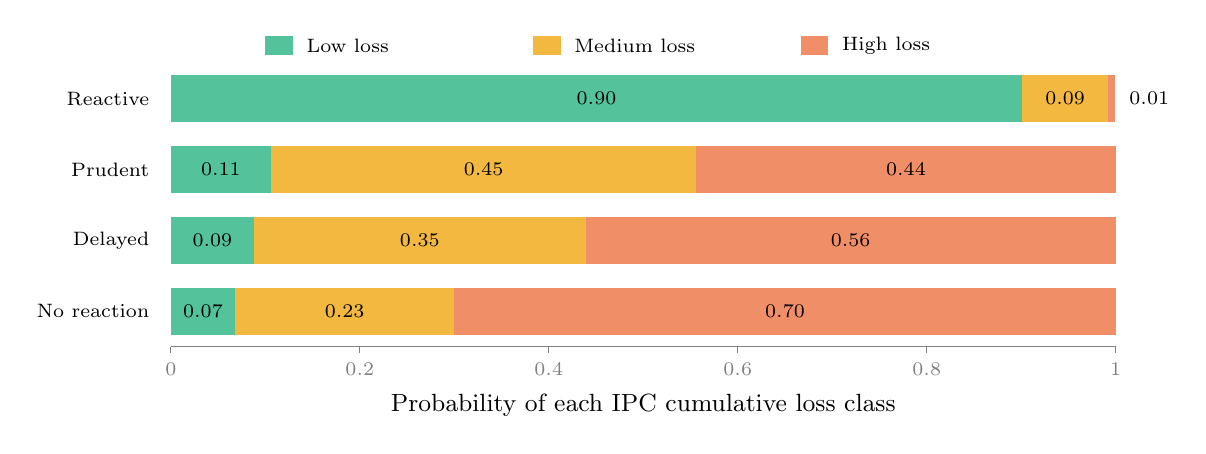
\begin{tikzpicture}[x=1cm,y=1cm, font=\scriptsize]
  \node[anchor=east] at (-0.15,0.00) {Reactive};
  \fill[palmec!75] (0.000,-0.30) rectangle (10.812,0.30);
  \node at (5.406,0.00) {$0.90$};
  \fill[poltard!75] (10.812,-0.30) rectangle (11.904,0.30);
  \node at (11.358,0.00) {$0.09$};
  \fill[polprud!75] (11.904,-0.30) rectangle (11.988,0.30);
  \node[anchor=west] at (12.05,0.00) {$0.01$};
  \node[anchor=east] at (-0.15,-0.90) {Prudent};
  \fill[palmec!75] (0.000,-1.20) rectangle (1.272,-0.60);
  \node at (0.636,-0.90) {$0.11$};
  \fill[poltard!75] (1.272,-1.20) rectangle (6.672,-0.60);
  \node at (3.972,-0.90) {$0.45$};
  \fill[polprud!75] (6.672,-1.20) rectangle (12.000,-0.60);
  \node at (9.336,-0.90) {$0.44$};
  \node[anchor=east] at (-0.15,-1.80) {Delayed};
  \fill[palmec!75] (0.000,-2.10) rectangle (1.056,-1.50);
  \node at (0.528,-1.80) {$0.09$};
  \fill[poltard!75] (1.056,-2.10) rectangle (5.268,-1.50);
  \node at (3.162,-1.80) {$0.35$};
  \fill[polprud!75] (5.268,-2.10) rectangle (12.000,-1.50);
  \node at (8.634,-1.80) {$0.56$};
  \node[anchor=east] at (-0.15,-2.70) {No reaction};
  \fill[palmec!75] (0.000,-3.00) rectangle (0.816,-2.40);
  \node at (0.408,-2.70) {$0.07$};
  \fill[poltard!75] (0.816,-3.00) rectangle (3.600,-2.40);
  \node at (2.208,-2.70) {$0.23$};
  \fill[polprud!75] (3.600,-3.00) rectangle (12.000,-2.40);
  \node at (7.800,-2.70) {$0.70$};
  \draw[black!50] (0,-3.15) -- (12.0,-3.15);
  \foreach \p/\l in {0/0,0.2/0.2,0.4/0.4,0.6/0.6,0.8/0.8,1/1} { \draw[black!50] (\p*12.0,-3.15) -- ++(0,-0.08) node[below] {$\l$}; }
  \node[font=\small] at (6.0,-3.90) {Probability of each IPC cumulative loss class};
  \fill[palmec!75] (1.20,0.55) rectangle (1.55,0.8); \node[anchor=west] at (1.60,0.675) {Low loss};
  \fill[poltard!75] (4.60,0.55) rectangle (4.95,0.8); \node[anchor=west] at (5.00,0.675) {Medium loss};
  \fill[polprud!75] (8.00,0.55) rectangle (8.35,0.8); \node[anchor=west] at (8.40,0.675) {High loss};
\end{tikzpicture}

\captionof{figure}{Prognosis of the cumulative loss by policy, for the long closure of a site located on a bottleneck: distribution of the three IPC classes inferred by the learned network.}\label{fig:d7}
\end{center}

Diagnosis sheds light on the opposite case, a high-loss crisis managed by a prudent profile. The network associates it with a long disruption, with a probability of 0.39 against 0.33 a priori, an almost certain use of inventory release (0.95), and an escalation to three or more levers (0.40 against 0.23 a priori). It thus points to a crisis that is too long for the chosen policy. The operations manager escalated, but starting from inventory levers whose effect wears off, without reaching rerouting in time. This diagnosis directs corrective action toward the policy, which should be more reactive or use a different order of levers, rather than toward the network.

Figure~6 of the main manuscript applies the backward reading of Section~3.4 of the main manuscript to the seven contexts that the ISOMORPH topology makes possible, for the objective of a low cumulative loss. The reactive profile is the most probable everywhere, and more so the longer the disruption lasts: its posterior probability rises from between 0.51 and 0.58 for a short disruption to between 0.72 and 0.79 for a long one. For a short disruption, the three other policies each retain between 0.12 and 0.18: a low loss remains attainable there without a rapid reaction, which is consistent with the sober recommendation of Section~4.3 of the main manuscript. The map, in contrast, varies little with the nature of the disruption and the target position, in line with the diagnosis, since in the learned structure these variables act on the loss only through the levers mobilized.

\subsection{Sensitivity to inventory cover}
\label{sec:S6.4}

The temporal representation makes it possible to study the role of inventories, which the main dataset neutralizes. On the ISOMORPH network, with its original travel times, 60 crises were simulated for each disruption nature and each cover, with no reaction from the operations manager, and we counted those that produce a visible drop in service (Figure~\ref{fig:d8} and Table~\ref{tab:S4}). The flow representation serves as the reference.

\begin{center}
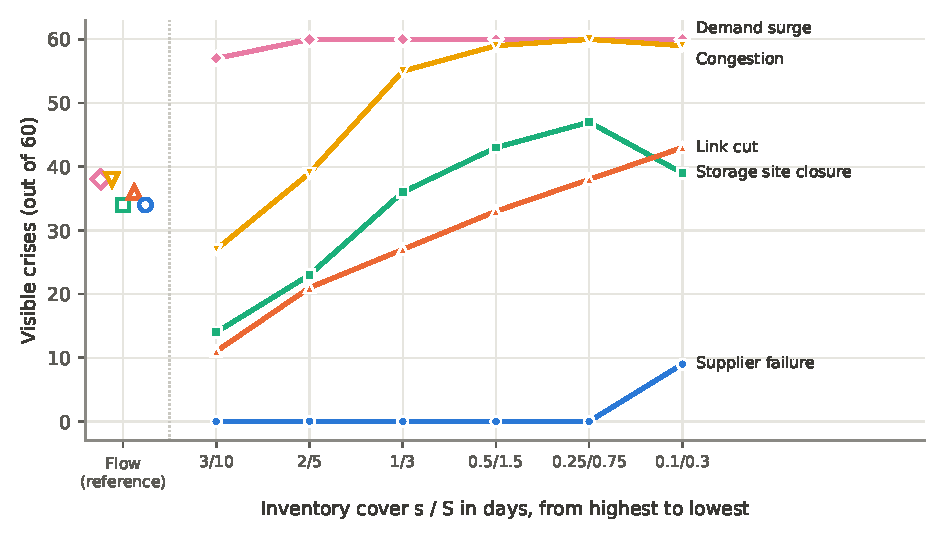
\includegraphics[width=0.75\textwidth]{figures/Fig8_inventory_cover_EN.pdf}
\captionof{figure}{Number of visible crises out of 60 by inventory cover, per disruption nature (ISOMORPH network, no reaction). The hollow symbols on the left give the reference of the flow representation.}\label{fig:d8}
\end{center}

For distribution disruptions (link cut, storage site closure and congestion), inventory cover acts as a gradual robustness lever: the lower it is, the more numerous the visible crises, from 11 to 43 out of 60 for a link cut and from 27 to 59 for a congestion. The boundary between robustness and resilience discussed in Section~S4.3 therefore shifts in a controlled way with the inventory level. Supplier failures, in contrast, are absorbed as soon as the cover reaches a quarter of a day, including failures lasting 15 to 60 days at the default cover: the calibration of demand bounds the shortfall during a failure, which a few days of inventory are enough to offset. Finally, the demand surge is better absorbed without inventories than with them: in the flow representation, any capacity margin instantly serves the additional demand, whereas with lead times this additional demand must first be drawn from inventories sized on the nominal throughput, which replenishment rebuilds only after a delay.

Inventory cover is therefore not a universal resilience lever. It protects against losses of distribution capacity, is almost superfluous against a small upstream failure, and does not protect against a demand shock, which calls for capacity or demand levers. These results, obtained with no reaction from the operations manager and with uniform cover, do not settle the question. The interaction between cover and management policy remains to be studied.

\begin{table}[htbp]
\caption{Crises producing a visible drop in service, out of 60, by inventory cover (ISOMORPH network, no reaction).}
\label{tab:S4}
\footnotesize
\begin{tabularx}{\textwidth}{@{}LLLLLLLL@{}}
\toprule
\textbf{Nature} & \textbf{Flow} & \textbf{3 / 10 d} & \textbf{2 / 5 d} & \textbf{1 / 3 d} & \textbf{0.5 / 1.5 d} & \textbf{0.25 / 0.75 d} & \textbf{0.1 / 0.3 d} \\
\midrule
Supplier failure & 34 & 0 & 0 & 0 & 0 & 0 & 9 \\
Link cut & 36 & 11 & 21 & 27 & 33 & 38 & 43 \\
Storage site closure & 34 & 14 & 23 & 36 & 43 & 47 & 39 \\
Demand surge & 38 & 57 & 60 & 60 & 60 & 60 & 60 \\
Congestion & 38 & 27 & 39 & 55 & 59 & 60 & 59 \\
\bottomrule
\end{tabularx}
\end{table}

\subsection{Detailed economic analysis and cost of overreaction}
\label{sec:S6.5}

The reactive policy is both the most effective and the most profitable per lever: each of its levers preserves on average 6,630 units, or about one third of a day of demand. For a margin of 10 euros per unit, it remains profitable as long as a lever costs less than 66,000 euros per crisis. The prudent policy, in contrast, is economically dominated: it engages more than two thirds of the levers of the reactive policy for a quarter of its gains. Each lever it adds to the delayed policy preserves only 790 units. The cost of a policy therefore depends less on the number of levers than on when they are engaged: engaged early, they prevent the crisis from lengthening; engaged late or in the wrong order, they arrive when most of the loss has already been incurred. Profitability also depends on the nature of the disruption: the break-even ratio of the reactive policy reaches 13,100 units per lever for a supplier failure, but only 2,300 for a congestion, which global levers mitigate poorly. The high break-even ratio of the delayed policy calls for a caveat: its gains come mainly from demand levers, in particular from the postponement of non-critical demand, which raises the measured service level by deferring sales rather than preserving them. Part of these gains is therefore carried over to the following period. Its break-even ratio is probably overestimated.

Figure~7 of the main manuscript draws the consequence for the choice of a policy. Among fixed policies, reactivity is optimal as long as the cost of a lever stays below the break-even ratio of 6,630 units of margin; beyond that, it is better not to react. The prudent and delayed policies are never the best choice. The dashed black curve selects, for each crisis and each lever cost, the policy with the best profit, then averages it over the 2,000 crises. This choice is made a posteriori, as if the outcome of each policy were known in advance: the curve is therefore an upper bound on what a crisis-specific recommendation can yield, of which the Bayesian network, which knows the crisis only partially, captures only a part. This upper bound keeps a positive profit well beyond the break-even ratio of the reactive policy, because for some crises the delayed policy or no reaction is sufficient. For a lever worth 5,000 units of margin, the crisis-specific choice would raise the average profit from 4,560 to 8,350 units per crisis, that is, 83\% more than the best fixed policy; for a more expensive lever, it would remain the only one to yield a gain. The recommendation of the Bayesian network targets precisely this value, by identifying, from what is known about a crisis, the cases where a more sober policy is sufficient.

Two additional batches, with the settings of the main batch, measure the cost of overreaction: 400 scenarios without any perceptible disruption and 300 minor disruptions (severity from 0.1 to 0.3, duration from 1 to 3 days). Without disruption, no profile engages a lever, because detection, based on the smoothed service level, is not triggered by demand fluctuations alone. In the face of a minor disruption, however, the reactive profile engages at least one lever in 32\% of cases, compared with 4\% for the prudent profile and none for the delayed profile, while reducing lost sales only from 2,335 to 2,260 units per crisis. Each lever there preserves about 230 units, nearly thirty times less than over all the crises of the main dataset. The sensitivity of the reactive profile therefore has a real cost in the face of minor disruptions, mostly demand surges and congestions: it is justified only if a minor disruption can be distinguished from a severe crisis, which is what the prognosis of the Bayesian network aims to do.

\section{Reproducibility of figures and tables}
\label{sec:S7}
\sloppy


This part indicates, for each figure derived from the data, how to reproduce it from the files deposited with the article and from the Isomorph-Reborn application.

\subsection*{ISOMORPH network (Figure~\ref{fig:d2})}

In the Isomorph-Reborn application, provided with the article, open the ``Générateur de scénarios'' (scenario generator) tab; in the ``Réseau'' (network) section, at the top of the tab, choose ``Réseau ISOMORPH'' (ISOMORPH network) to display the echelon diagram of Figure~\ref{fig:d2}. The description of the network, with its capacities and travel times, is contained in the file \texttt{reseau\_isomorph-originel.json}.

\subsection*{Crisis S0366 under the four policies (Figure~2 of the main manuscript)}

In the ``Générateur de scénarios'' tab of Isomorph-Reborn, load the assumptions file \texttt{hypotheses\_lot} \texttt{\_A\_isomorph\_tension75.json} (ISOMORPH network, flow representation, strain level 75, 2,000 scenarios, seed 42) and run the generation. The daily trajectories are exported to the file \texttt{ip\_timeseries.csv} (columns \texttt{scenario\_id}, \texttt{branch\_id}, \texttt{day\_rel} and \texttt{ip}); Figure~2 of the main manuscript shows the four versions of scenario S0366. The detection days come from the learning dataset exported for the same batch.

\subsection*{Fit of crisis S0366 (Figure~3 of the main manuscript)}

The fitted parameters of each crisis version are exported by Isomorph-Reborn (``Ajustement par lot'' (batch fitting) tab) to the file \texttt{resilience\_ip.csv} (columns \texttt{k}, \texttt{q}, \texttt{h}, \texttt{g}, \texttt{d}, \texttt{alpha}, \texttt{beta}, \texttt{r2}, followed by the six indicators). The plotted curve is Eq.~(2) of the main manuscript evaluated with the parameters of row S0366, version \texttt{none}, superimposed on the trajectory from the file \texttt{ip\_timeseries.csv}. In the application, this crisis is curve no.~1461 of 8,000: the counter numbers the crisis versions, four per scenario, and not the scenarios.

\subsection*{Bayesian network learning (Figure~5 of the main manuscript)}

In BayesArtist, import the dataset \texttt{bayesartist\_apprentissage\_lotA.csv} (6,400 crisis versions, 20 variables) and the constraints \texttt{bayesartist\_contraintes\_isomorph.json} (155 forbidden arcs, at most four parents), then run learning by greedy search (\textit{Greedy Hill Climbing}) with the BIC score and Laplace smoothing. The learned network is exported in \texttt{.bif} format; the figure is drawn from this file. Since BayesArtist is not publicly distributed, the same learning can be carried out with any Bayesian network software that learns from a CSV file and accepts forbidden arcs (see the data availability statement of the main manuscript).

\subsection*{Prognosis for the case study (Figure~\ref{fig:d7})}

In BayesArtist, in inference mode on the network of Figure~5 of the main manuscript, set the evidence nature = \texttt{fermeture\_entrepot}, target = \texttt{passage\_oblige} and duration = \texttt{fort}, then successively set the profile to \texttt{none}, \texttt{tardif}, \texttt{prudent} and \texttt{reactif} and read the distribution of the IPC node each time.

\subsection*{Recommendation map (Figure~6 of the main manuscript)}

In BayesArtist, on the network of Figure~5 of the main manuscript, set the nature, target and duration evidence corresponding to a context of the map, together with IPC = \texttt{faible}, then read the distribution of the profile node. The map is computed by exact inference on the network exported in \texttt{.bif} format; BayesArtist, whose inference is approximate, gives the same values to within 0.01 (for example 0.06, 0.08, 0.10, and 0.76 for the long closure of a bottleneck).

\subsection*{Economic analysis (Table~8 and Figure~7 of the main manuscript)}

Lost sales are computed from the file \texttt{ip\_timeseries.csv} of batch A, as the sum of $1 - \mathrm{PI}(t)$ over the 60 days following the disruption multiplied by the reference demand; the number of levers engaged and the reference demand come from the learning dataset exported for the same batch (columns \texttt{nb\_decisions} and \texttt{base\_demand}).


\bibliographystyle{cas-model2-names}
\bibliography{references}

\end{document}
